\begin{enumerate}
  \item Sea $f(k)$ el mínimo número de operaciones para obtener $k$ empezando desde $1$, para $k \ge 1$.

  \[
  f(k) =
  \begin{cases}
  0 & \text{si } k = 1 \\
  1 + \min\big(f(k-1),\ [k \text{ par}]\ f(k/2),\ [k \equiv 0 \!\!\pmod 3]\ f(k/3)\big) & \text{si } k > 1
  \end{cases}
  \]

  donde un candidato solo participa en el $\min$ si su condición ($k$ par, o $k$ múltiplo de $3$) se cumple. La respuesta al problema es $f(n)$.

  \begin{itemize}
    \item $f(k)$: mínimo número de operaciones para llegar a $k$ desde $1$.
    \item $k$: el número que se quiere alcanzar en este subproblema (no necesariamente el $n$ de la entrada).
    \item Cada candidato del $\min$ corresponde a deshacer la \emph{última} operación aplicada para llegar a $k$: si fue ``sumar $1$'', antes se estaba en $k-1$; si fue ``multiplicar por $2$'', antes se estaba en $k/2$ (solo posible si $k$ es par); si fue ``multiplicar por $3$'', antes se estaba en $k/3$ (solo si $k$ es múltiplo de $3$). Se toma la que resulte en menos operaciones.
  \end{itemize}

  \pagebreak

  \item El grafo de dependencias tiene un vértice por cada $k \in \{1,\ldots,n\}$, con un eje entrante desde $k-1$ (siempre), desde $k/2$ (si $k$ es par) y desde $k/3$ (si $k$ es múltiplo de $3$):

\begin{center}
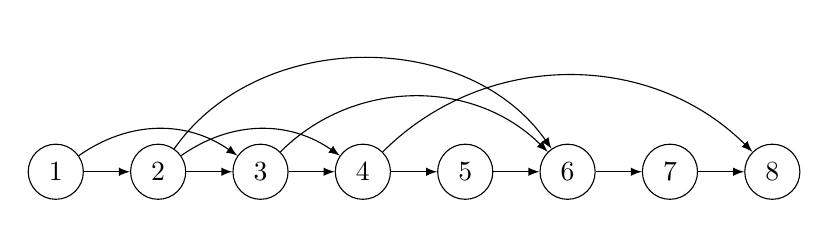
\begin{tikzpicture}[
  vertex/.style={circle, draw, minimum size=0.7cm, inner sep=0pt},
  -latex,
]
  \foreach \k in {1,...,8} {
    \node[vertex] (n\k) at (1.3*\k, 0) {\k};
  }

  \draw (n1) to (n2);
  \draw (n2) to (n3);
  \draw (n3) to (n4);
  \draw (n4) to (n5);
  \draw (n5) to (n6);
  \draw (n6) to (n7);
  \draw (n7) to (n8);

  \draw (n1) to[bend left=35] (n3);
  \draw (n2) to[bend left=35] (n4);
  \draw (n3) to[bend left=45] (n6);
  \draw (n2) to[bend left=55] (n6);
  \draw (n4) to[bend left=45] (n8);
\end{tikzpicture}

Dependencias entre $1$ y $8$: la cadena inferior es siempre $k-1 \to k$; los arcos superiores son $k/2 \to k$ y $k/3 \to k$ cuando aplican (e.g., $3\to6$ y $2\to6$ porque $6/2=3$ y $6/3=2$).
\end{center}

  A diferencia de una recurrencia por capas (donde $k$ solo depende de $k-1$), aquí $k/2$ y $k/3$ pueden estar arbitrariamente lejos de $k$ (e.g., $k=2^{20}$ depende de $k/2 = 2^{19}$). Por eso no basta con recordar una ``capa'' anterior: cualquier $f(j)$ con $j<k$ puede ser consultado por un $k$ mucho más grande más adelante, así que hay que conservar la tabla completa. Una solución de programación dinámica requiere, entonces, $\Theta(n)$ de espacio como mínimo.

  \pagebreak

  \item Tabulación bottom-up en Python, calculando $f$ en orden creciente de $k$ (space $\Theta(n)$, tiempo $\Theta(n)$, pues cada $f(k)$ se resuelve con trabajo $\Theta(1)$):

\begin{pseudocode}
def min_operaciones(n: int) -> int:
    f = [0] * (n + 1)
    for k in range(2, n + 1):
        f[k] = f[k - 1] + 1
        if k % 2 == 0:
            f[k] = min(f[k], f[k // 2] + 1)
        if k % 3 == 0:
            f[k] = min(f[k], f[k // 3] + 1)
    return f[n]
\end{pseudocode}
\end{enumerate}
